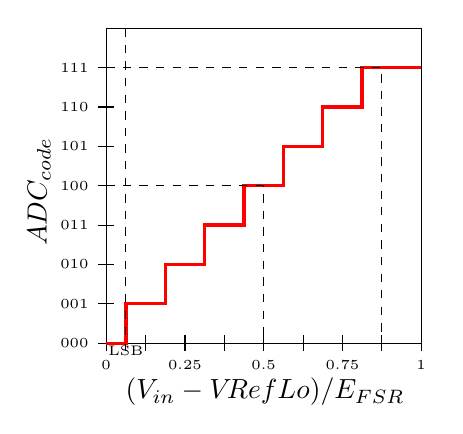
\begin{tikzpicture}
\tikzstyle{stealth} = [-stealth, thick]
\tikzstyle{invisible} = [outer sep=0,inner sep=0,minimum size=0]
\tikzstyle{circle} = [shape=circle, minimum size=0.5cm, draw=black!55]
\tikzstyle{line} = [draw, very thick, red]

\draw (0,0) node [invisible] (v1) {} --
	  (4,0) node [invisible] {} --
	  (4,4) node [invisible] {} --
	  (0,4) node [invisible] {} --
	  (0,0) node [invisible] {};
\foreach \x in {0,0.25,0.5,0.75,1}
		{
			\draw (\x*4,-0.1)node [below,font=\tiny,] {\x } -- (\x*4,0.1) ;
		}
\foreach \x in {0.125,0.375,0.625,0.875,1}
		{
			\draw (\x*4,-0.1)node [below,font=\tiny,] {} -- (\x*4,0.1);
		}
\foreach \c [count=\x from 0] in {{000},{001},{010},{011},{100},{101},{110},{111}}
{
	\draw (-0.1,\x*0.5)node [anchor=east,font=\tiny,] {\c} -- (0.1,\x*0.5);
}
        %\node at (0,\x) {\c};	
\draw [line](v1) -- (0.25,0) node [invisible] {} -- 
		(0.25,0.5) node [invisible] {} -- 
		(0.75,0.5) node [invisible] {} -- 
		(0.75,1) node [invisible] {} -- 
		(1.25,1) node [invisible] {} -- 
		(1.25,1.5) node [invisible] {} -- 
		(1.75,1.5) node [invisible] {} -- 
		(1.75,2) node [invisible] {} -- 
		(2.25,2) node [invisible] {} -- 
		(2.25,2.5) node [invisible] {} -- 
		(2.75,2.5) node [invisible] {} -- 
		(2.75,3) node [invisible] {} -- 
		(3.25,3) node [invisible] {} -- 
		(3.25,3.5) node [invisible] {} -- 
		(4,3.5) node [invisible] {};
\node [invisible] at (2.0187,-0.6198) {$(V_{in}-V_{}RefLo)/E_{FSR}$};
\node [invisible, rotate=90] at (-0.8509,1.9232) {$ADC_{code}$};
\draw [dashed](0,2) node [invisible] {} -- (2,2) node [invisible] {} -- (2,0) node [invisible] {};
\draw [dashed](0,3.5) node [invisible] {} -- (3.5,3.5) node [invisible] {} -- (3.5,0) node [invisible] {};
\draw [dashed](0.25,4) node [invisible] {} -- (0.25,-0.1) node [invisible] {\tiny LSB};
\end{tikzpicture}






